\begin{figure}[htbp]\centering
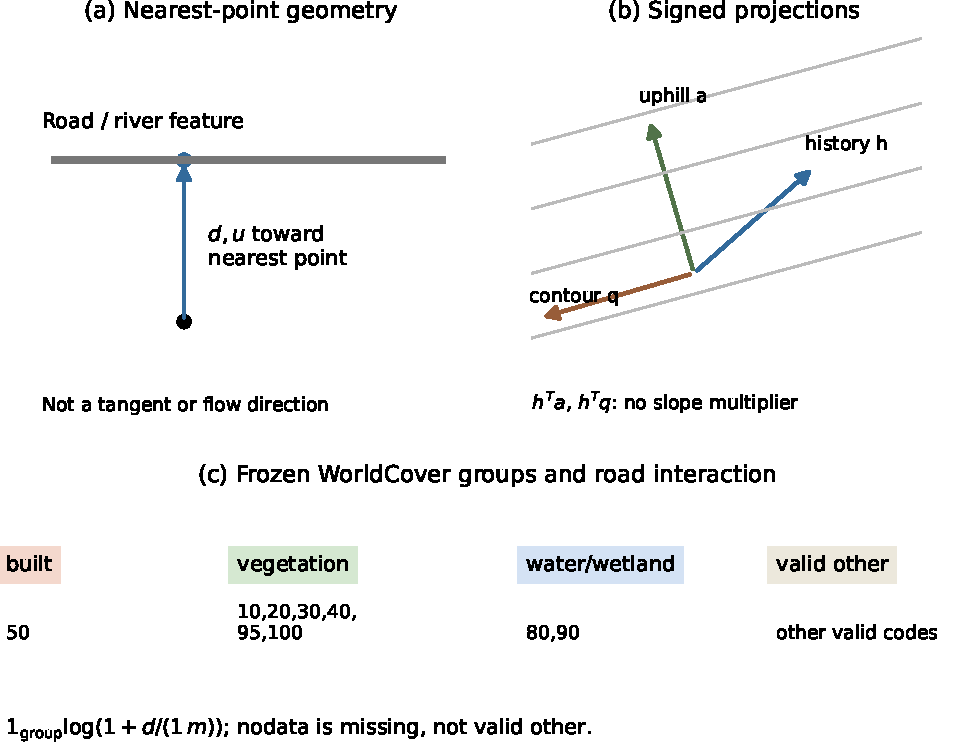
\includegraphics[width=\linewidth]{../figures/reader-v2/geometry.pdf}
\caption{输入几何：三个示意面板，不含实测效应。距离与方向指向最近要素点；
带符号上坡／等高线投影不乘坡度。坡度大小是另一个输入，本图未绘出。
冻结WorldCover分组为建筑50，植被10/20/30/40/95/100，水体／湿地80/90，
以及其他有效代码。无效或nodata值作为缺失，不归入“其他”。}
\label{fig:input-geometry}\end{figure}

\begin{figure}[htbp]\centering
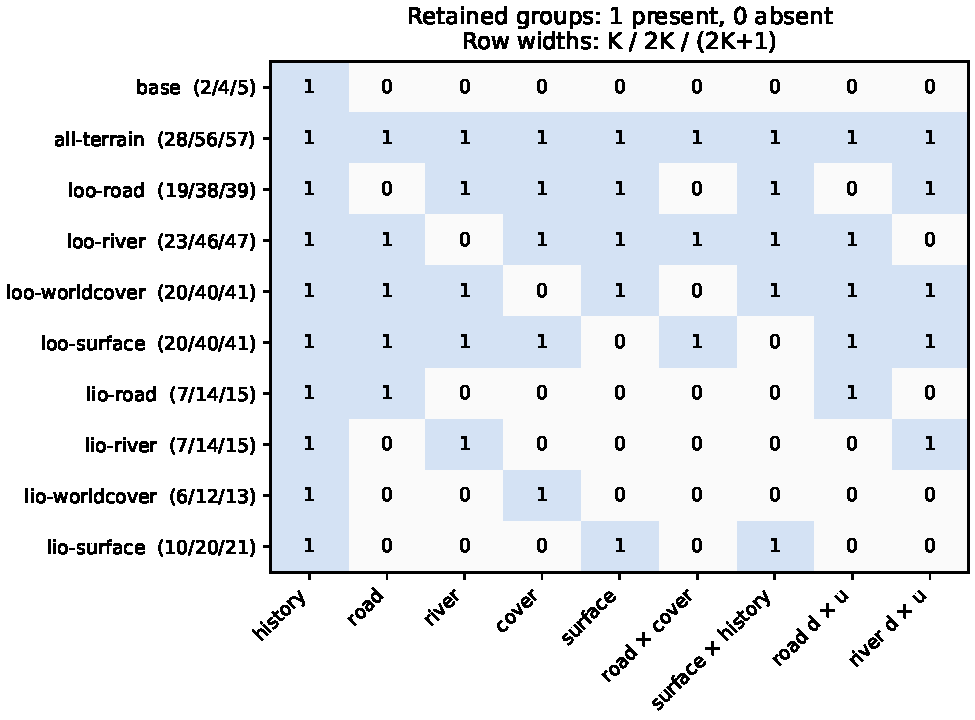
\includegraphics[width=\linewidth]{../figures/reader-v2/design.pdf}
\caption{十配置乘九组／依赖列，共90设计状态格，不是实测数据。
$K$为数值特征数，$2K$含对应掩码，$2K+1$再含截距；这些不是拟合秩或自由度。
每行保留历史。道路--覆盖依赖两个父组，坡面--历史在LIO-surface仍保留。}
\label{fig:input-design}\end{figure}
整体比较是all-terrain减base；移除一组（LOO）比较all-terrain与all-minus-group，
只加入一组（LIO）比较history-plus-group与base。
候选减对照的评分负差有利于候选；若把移除损失写成因素收益，则须反转符号，
区间$[l,u]$变为$[-u,-l]$。图\ref{fig:input-design}的依赖列说明，
移除一组可能同时删除多个数值特征。即使必需失败使地形推断不可用，
这些设计定义仍明确说明了试验原本比较什么。
\FloatBarrier
